Hier werden die einzelnen Technologien beschrieben, die für die Applikation verwendet wurden, zuerst Softwarekomponenten, danach die Entwicklungsinfrastruktur.

\section{Java}
\setauthor{Hain Lukas}

Das Backend dieser Applikation wurde in der Programmiersprache Java entwickelt.
Java ist nicht nur eine Programmiersprache, sondern ebenso ein Laufzeitsystem, was Oracle durch den Begriff Java Platform verdeutlichen will. 
So gibt es neben der Programmiersprache Java durchaus andere Sprachen, die eine Java-Laufzeitumgebung ausführen, etwa diverse Skriptsprachen wie 
Groovy, JRuby, Jython, Kotlin oder Scala. Skriptsprachen auf der Java-Plattform werden immer populärer; sie etablieren eine andere Syntax, nutzen aber die JVM und die Bibliotheken.
Zu der Programmiersprache und JVM kommt ein Satz von Standardbibliotheken für Datenstrukturen, Zeichenkettenverarbeitung, Datum/Zeit-Verarbeitung, grafische Oberflächen, 
Ein-/Ausgabe, Netzwerkoperationen und mehr. Das bildet die Basis für höherwertige Dienste wie Datenbankanbindungen oder Webservices. Integraler Bestandteil der Standardbibliothek 
seit Java 1.0 sind weiterhin Threads. Sie sind leicht zu erzeugende Ausführungsstränge, die unabhängig voneinander arbeiten können. 
Mittlerweile unterstützen alle populären Betriebssysteme diese »leichtgewichtigen Prozesse« von Haus aus, sodass die JVM diese parallelen Programmteile nicht nachbilden muss, 
sondern auf das Betriebssystem verweisen kann. Auf den neuen Multi-Core-Prozessoren sorgt das Betriebssystem für eine optimale Ausnutzung der Rechenleistung, da Threads wirklich nebenläufig arbeiten können.
\cite{sysarch-java-1}

\section{Quarkus}
\setauthor{Hain Lukas}

Die Programmiersprache alleine reicht allerdings für eine Web-API noch nicht aus, desshalb wird im Backend das Quarkus Framework mit den Libraries RESTEasy und Hibernate ORM verwendet.
Quarkus ist ein Kubernetes-natives Full-Stack Java Framework für JVMs (Java Virtual Machines) und native Kompilierung, mit dem Java speziell für Container optimiert wird. 
Es bietet eine effektive Plattform für Serverless-, Cloud- und Kubernetes-Umgebungen. Quarkus wurde speziell für 
beliebte Java-Standards, Frameworks und Libraries wie RESTEasy (JAX-RS) und Hibernate ORM (JPA), die wie oben erwähntin der Applikation verwendet werden, 
sowie für Apache Kafka, Eclipse MicroProfile, Spring, Infinispan, Camel und viele mehr konzipiert.
Die Dependency-Injection-Lösung von Quarkus basiert auf CDI (Contexts and Dependency Injection) und bietet ein Framework, mit dessen Hilfe die Funktionalität 
erweitert und ein Framework konfiguriert, gebootet und in Ihre Anwendung integriert werden kann. 

Quarkus wurde als benutzerfreundliches Tool konzipiert und integriert Funktionen, die keine oder nur wenig Konfiguration erfordern.
Entwickler können die passenden Java Frameworks für ihre Anwendungen auswählen, die dann im JVM-Modus laufen oder kompiliert und im nativen Modus ausgeführt werden können.
Das ganz auf Entwickler abgestimmte Quarkus integriert außerdem folgende Funktionen:
\begin{itemize}
    \item Live-Codierung zur umgehenden Prüfung der Auswirkungen von Code-Änderungen sowie eine schnelle Problembehebung
    \item Einheitliche imperative und reaktive Programmierung mit einem eingebetteten gemanagten Event Bus
    \item Einheitliche Konfiguration
    \item Einfaches Generieren nativer Programmdateien
\end{itemize}
Ob man die Anwendungen auf einer Public Cloud oder in einem intern gehosteten Kubernetes-Cluster hosten, Eigenschaften wie ein schneller 
Start sowie ein niedriger Speicherverbrauch sind wichtig, um die Gesamtkosten für das Hosting niedrig zu halten.
Quarkus wurde auf Basis einer Container-first-Philosophie entwickelt und soll so einen niedrigen Speicherverbrauch und schnelle Startzeiten auf folgende Weise ermöglichen:
\begin{itemize}
    \item Erstklassiger Support für Graal/SubstrateVM
    \item Metadaten-Verarbeitung gleichzeitig mit dem Build
    \item Reduzierung der Reflektionsnutzung
    \item Preboot nativer Images
\end{itemize}
Bei der Anwendungsentwicklung mit Quarkus wird im Vergleich zum traditionellen Java nur ein Zehntel des Speichers belegt. Dazu bietet es bis zu 300 Mal 
schnellere Startzeiten. Beide Aspekte ermöglichen eine deutliche Reduzierung der Kosten für Cloud-Ressourcen.
Quarkus ist so konzipiert, dass bei der Anwendungsentwicklung der bewährte imperative Code problemlos mit dem nicht-blockierenden reaktiven Code kombiniert werden kann.
Dies erweist sich als nützlich sowohl für Java-Entwickler, die an das imperative Modell gewöhnt sind und auch dabei bleiben möchten, und all diejenigen, die einen cloudnativen/reaktiven Ansatz bevorzugen.
Das Quarkus-Entwicklungsmodell lässt sich flexibel an alle zu erstellenden Anwendungstypen anpassen.
Quarkus ist eine effiziente Lösung zur Ausführung von Java in dieser neuen Welt von Serverless-Architekturen, Microservices, Containern, Kubernetes, 
Function-as-a-Service (FaaS) und Clouds, weil es für all diese Technologien entwickelt wurde.
\cite{sysarch-quarkus-1}

\subsection{RESTEasy}

RESTEasy ist ein JBoss/Red Hat-Projekt, das verschiedene Frameworks zur Verfügung stellt, die bei der Erstellung von RESTful Web Services und RESTful Java-Anwendungen unterstützen, 
und es ist die Schnittstelle zwischen dem Frontend und Backend der Applikation. 
Es ist eine Implementierung der Jakarta RESTful Web Services, einer Spezifikation der Eclipse Foundation, die eine Java-API für RESTful Web Services über das HTTP-Protokoll bereitstellt.
Darüber hinaus implementiert RESTEasy auch die MicroProfile REST Client Spezifikation API.

RESTEasy kann in jedem Servlet-Container ausgeführt werden, aber eine engere Integration mit WildFly Application Server und Quarkus 
ist ebenfalls verfügbar, um die Benutzerfreundlichkeit in diesen Umgebungen zu verbessern.
\cite{sysarch-quarkus-2}

\subsection{Hibernate ORM with Panache}

Hibernate ORM ist die Schnittstelle zwischen Backend und Datenbank. Bei Hibernate handelt es sich um ein Framework zur Abbildung von Objekten auf relationalen Datenbanken für die Programmiersprache Java - es wird auch als Object Relational Mapping Tool bezeichnet. 
Hibernate ist in der Programmiersprache Java implementiert und steht als Open Source zur freien Verfügung. Hibernate nutzt das Konzept der Reflexion, um so zur Laufzeit einer Software sogenannte 
Meta- Informationen über die Struktur von Objekten und die zugrunde liegenden Klassen zu ermitteln, die dann auf die Tabellen einer Datenbank abgebildet werden.
\cite{sysarch-quarkus-3}

Object Relational Mapping (ORM) ist eine Programmiertechnik zur Konvertierung von Daten zwischen relationalen Datenbanken und objektorientierten Programmiersprachen. 
Mit der ORM-Technik können Objekte auf die Strukturen einer relationalen Datenbank abgebildet werden.
\cite{sysarch-quarkus-4}

\subsection{Apache Maven}

Als Build-Tool wird im Quarkus Backend Apache Maven verwendet. Maven wurde von der Apache Software Foundation für die Projektverwaltung entwickelt. 
Entwickler können damit Java-Projekte automatisieren. Maven ist ein Teil der Apache Software Foundation und wird von dieser gehostet. 
Das Tool ist aus einem Teil des Jakarta-Projekts hervorgegangen. Maven vereinfacht den Softwareerstellungsprozess, bietet ein einheitliches System für die Entwicklerarbeit, hochwertige Projektinformationen, 
Richtlinien für das Festlegen von Best Practices und erleichtert die Migration zu neuen Funktionen durch mehr Transparenz. Maven beschreibt sowohl, wie Software gebaut wird, als auch deren Abhängigkeiten. 
Apache hilft sowohl bei der Verwaltung von Projekten und dient als Tool zum Verständnis. Es hilft also dabei, den Zustand eines Projekts sehr schnell darzustellen.
Das Programm wird von Entwicklern und Projektmanagern von Java-Anwendungsprojekten verwendet. Das Tool kann nützlich sein, um den aktuellen Zustand eines Projektes 
auf einem Blick für technisch weniger versierte Personen, wie Führungspersönlichkeiten und Investoren, zusammenzufassen. Maven basiert auf dem Objektmodell. 
Projekte werden als eine Pom.xml-Datei gespeichert. 

Das Tool verwaltet Projekt-Builds, Reporting und Dokumentation aus der zentralen XML-Informationsbasis. 
Mit seiner Standard-Plug-in-Architektur kann Maven über Standard-Input mit so gut wie jeder Anwendung zusammenarbeiten.
Maven vereinfacht den Prozess für das Erstellen von Java-Anwendungen erheblich, da Nutzer den Status des Projektes viel einfacher einschätzen können.
Der Name Maven kommt aus dem Jiddischen und bedeutet Akkumulator von Wissen. Obwohl Maven das Entwickeln von Software anhand von Konventionen ermöglicht, 
sind reproduzierbare Builds derzeit kein Feature. Die Entwickler arbeiten aber daran. 
\cite{sysarch-maven-1}

\section{PostgreSQL}
\setauthor{Hain Lukas}

Die Datenbank der Wahl ist in dieser Diplomarbeit die PostgreSQL Datenbank, da die Diplomanden im Unterricht bereits erfahrung damit angesammelt haben.
Dieses DBMS (Datenbank-Managementsystem) bietet eine liberale Lizenz, flexiblen Umgang mit Datentypen, ist skalierbar und vielseitig nutzbar.
Der Definition nach ist PostgreSQL ein „objektrelationales“ Datenbank-Managementsystem (DBMS). Es ist Open Source und orientiert sich sehr eng am SQL-Standard. Bestehende SQL-Anwendungen 
können durch den ANSI-SQL-Standards ohne großen Aufwand integriert werden. Die Funktionsweise entspricht dem klassischen Client-Server-Prinzip, bei dem unterschiedliche Clients Anfragen an den Datenbankserver senden.
In der Praxis ist es mit PostgreSQL möglich, komplexere Anwendungen und Workloads zu entwickeln und zu betreiben als mit anderen Lösungen. 
Es unterstützt eine Vielzahl Datentypen und Operatoren. Entwickler können hier bei Bedarf eigene Datentypen definieren. PostgreSQL ist nicht nur für Webanwendungen sehr gut geeignet, es kann auch große Enterprise-Datenbanken abbilden. 
PostgreSQL findet auch in Desktop-Systemen Einsatz: Es ist das Datenbanksystem von Linux und macOS. Diese Systeme liefern das Datenbanksystem standardmäßig mit.
\cite{sysarch-postgresql-1}

\subsection{Offene Lizenz}
PostgreSQL hat eine Offene Lizenz. Es ist unter der eigenen PostgreSQL-Lizenz veröffentlicht. Generell fallen dabei keine Lizenzkosten an. 
Diese liberale Lizenz erlaubt es, das System beliebig zu vertreiben. Änderungen müssen nicht der Community zur Verfügung gestellt werden. Die Verwendung von PostgreSQL hat 
keine nachgelagerten Auswirkungen darauf, wie Weiterentwicklungen und darauf basierende Lösungen verwendet werden dürfen oder veröffentlicht werden müssen.
\cite{sysarch-postgresql-1}

\subsection{Großes Potenzial}

Die Datenbankgröße ist nicht durch das System begrenzt, sondern nur durch den zur Verfügung stehenden Speicher. Da Postgres flexibel und kompatibel aufgebaut ist, 
können eine Vielzahl an Anwendungen auf diese Datenbanklösung bauen. Dazu bietet PostgreSQL die Möglichkeit, 
Trigger einzusetzen und bietet Schnittstellen zu vielen verschiedenen Programmiersprachen, was den Einsatzzweck und die Zusammenarbeit mit unterschiedlichsten Anwendungen potenziell vielfältig macht.
\cite{sysarch-postgresql-1}

\subsection{Sichere Replikation}

Ein weiterer Punkt ist die detaillierte Zugriffskontrolle und sichere Datenreplikation. In der Praxis ist je nach Anwendungsfall asynchrone oder synchrone Replikation möglich: 
Synchrone Replikation, um sicherzustellen, dass kritische Transaktionen auf beiden Servern ausgeführt wurden. Asynchrone Replikation für maximale Geschwindigkeit bei weniger kritischen Transaktionen. 
Ein weiterer Vorteil ist die freie Wahl der Hardware und des Server-OS. PostgreSQL kann auf diversen Linux-Distributionen, BSD, Windows oder macOS 
gehostet werden.
\cite{sysarch-postgresql-1}

\section{KeyCloak}
\setauthor{Hain Lukas}

Zum verwalten von Userdaten wird in dieser Applikation ein KeyCloak Server verwendet.
Keycloak ist eine Open-Source-Lösung für Identity und Access Management (IAM), die auf die Entwicklung moderner Anwendungen und Services ausgerichtet ist.
\cite{sysarch-keycloak-1}

\subsection{Single Sign-on und Single Sign-out}

Möchte man mehrere Applikationen oder Dienste verwenden, so sind in der Regel bei jeder Applikation separate Logins erforderlich. Beim Single Sign-on (SSO) geht es jedoch darum, 
dass nur eine einzige Authentifizierung notwendig ist (beim ersten Zugriff auf eine der Applikationen). Dies geschieht dadurch, dass die Applikation die Benutzerin bzw. 
den Benutzer auf eine zentrale Keycloak-Instanz weiterleitet, welche die Login-Maske für die angesprochene Applikation ausgibt und in der Folge die Authentifizierung durchführt.
Nach erfolgreicher Anmeldung wird zur Applikation weitergeleitet. Werden anschließend andere Software-Systeme im SSO-Verbund verwendet, dann weiß Keycloak, dass die Benutzerin bzw. 
der Benutzer bereits authentifiziert ist und fordert keine weitere Anmeldung mehr. Zusätzlich verfügt Keycloak auch über eine Kerberos-Bridge, sodass die Anmeldung am Arbeitsrechner 
für die Authentifizierung ausreicht. Darüber hinaus unterstützt Keycloak auch ein Single Sign-out: Nach der Abmeldung erfolgt das automatische Ausloggen aus allen Applikationen im SSO-Verbund.
\cite{sysarch-keycloak-2}

\subsection{Unterstützung von Standardprotokollen}

Keycloak unterstützt Standardprotokolle wie OAuth 2.0 (nur Autorisierung) und das darauf basierende OpenID Connect (Autorisierung und Authentifizierung). 
Daneben wird mit SAML 2.0 ein weiteres Standardprotokoll unterstützt, welches ähnliche Anforderungen wie OpenID Connect (OIDC) abdeckt. 
Im Gegensatz zu OIDC existiert SAML jedoch schon länger, basiert auf XML und setzt zum Erreichen von Integrität und Vertraulichkeit digitale Signaturen und entsprechende Zertifikate ein.
\cite{sysarch-keycloak-2}

\subsection{Account Management Console}

Ein Self-Service-Portal ermöglicht es Benutzern, ihre Daten jederzeit selbst zu verwalten. Keycloak bietet ein solches Portal unter dem Namen „Account Management Console“ an. 
So können z. B. Passwortänderungen selbständig durchgeführt werden, ohne von Administratoren abhängig zu sein.
\cite{sysarch-keycloak-2}

\subsection{Admin Console}

Die Admin Console umfasst im Wesentlichen die Konfiguration von:
\begin{itemize}
    \item Realms (jeweils abgegrenzte Bereiche, für die die anderen in dieser Aufzählung genannten Aspekte einzeln konfiguriert bzw. verwaltet werden können)
    \item Clients (Applikationen und Dienste)
    \item Benutzerdatenquellen (siehe User Federation)
    \item weiteren Identity Providern (siehe Identity Brokering und Social Login)
    \item die Verwaltung von lokal in Keycloak angelegten Benutzern, Benutzern aus anderen Datenquellen, Benutzergruppen und Rollen
\end{itemize}
\cite{sysarch-keycloak-2}

\subsection{Client-Adapter}

Clients kommunizieren über die angebotenen Standardprotokolle mit Keycloak. Damit diese Kommunikation nicht für jeden Client – evtl. sogar redundant – selbst implementiert werden muss, 
gibt es für eine Vielzahl an Technologien und Frameworks fertige Client-Adapter, die sich einfach in die eigene Anwendung integrieren lassen und die Kommunikation mit Keycloak übernehmen. 
\cite{sysarch-keycloak-2}

\section{Docker}
\setauthor{Hain Lukas}

Um die Applikation unabhängig von Betriebsystem benutzen zu können, werden das Quarkus Backend, das Frontend, der KeyCloak Server sowie 
eine PostgreSQL Datenbank für Turnierdaten und eine für Userdaten jeweils in Docker Containern ausgeführt.
Die Docker-Technologie verwendet den Linux Kernel und seine Funktionen wie Cgroups und namespaces, um Prozesse zu isolieren, damit diese unabhängig voneinander ausgeführt werden können. 
Diese Unabhängigkeit ist der Zweck der Container – die Fähigkeit, mehrere Prozesse und Apps getrennt voneinander betreiben zu können. 
So wird die Infrastruktur besser genutzt und gleichzeitig die Sicherheit bewahrt, die sich aus der Arbeit mit getrennten Systemen ergibt.
Containertools, einschließlich Docker, arbeiten mit einem Image-basierten Bereitstellungsmodell. Das macht es einfacher, eine Anwendung oder ein Paket von Services mit all deren 
Abhängigkeiten in mehreren Umgebungen gemeinsam zu nutzen. Docker automatisiert außerdem die Bereitstellung der Anwendung 
(oder Kombinationen von Prozessen, die eine Anwendung darstellen) innerhalb dieser Container-Umgebung. Diese Tools bauen auf Linux-Containern auf 
und geben den Nutzern so nie dagewesenen Zugriff auf Anwendungen. Sie ermöglichen eine deutlich schnellere Bereitstellung und Kontrolle von Versionen sowie deren Verbreitung.
\cite{sysarch-docker-1}

\subsection{Vorteile}

\subsubsection{Modularität}

Der Docker-Ansatz für die Containerisierung konzentriert sich darauf, nur einen Teil der Anwendung für eine Reparatur oder Aktualisierung außer Betrieb zu nehmen, 
ohne dass die gesamte Anwendung außer Betrieb genommen werden muss. Zusätzlich zu diesem auf Microservices basierenden Ansatz können Sie Prozesse 
in mehreren Apps gemeinsam verwenden – so ähnlich wie bei einer serviceorientierten Architektur (SOA).
\cite{sysarch-docker-1}

\subsubsection{Layer und Image-Versionskontrolle}

Jedes Docker-Image besteht aus einer Reihe von Layern. Diese Layer werden in einem einzelnen Image vereint. Wenn sich das Image ändert, wird ein Layer erstellt. 
Jedes Mal, wenn ein Nutzer einen Befehl wie run oder copy eingibt, wird ein neuer Layer erstellt. Mit Docker werden diese Layer für neuer Container wiederverwendet, 
was die Entwicklung enorm beschleunigt. Zwischenzeitliche Änderungen werden von den Images gemeinsam verwendet, was die Geschwindigkeit, Größe und Effizienz weiter verbessert. 
Versionskontrolle ist ein fester Bestandteil des Layering. Bei jeder neuen hat man im Prinzip ein eingebautes Änderungsprotokoll und damit volle Kontrolle über die Container-Images.
\cite{sysarch-docker-1}

\subsubsection{Rollback}

Das Beste am Layering ist wahrscheinlich das Rollback, also das Zurücksetzen auf die vorherige Version. Jedes Image hat Layers. Wenn man mit der aktuellen Iteration eines Image nicht zufrieden ist, kann man einfach
auf die vorherige Version zurücksetzen. Dieser Ansatz unterstützt eine agile Entwicklung und sorgt, was die Tools angeht, 
für eine kontinuierliche Integration und Bereitstellung (Continuous Integration/Continuous Deployment - CI/CD).
\cite{sysarch-docker-1}

\subsubsection{Schnelle Bereitstellung}

Neue Hardware bereitzustellen und zum Laufen zu bringen, dauerte normalerweise Tage und war mit einem enormen Aufwand verbunden. Mit Docker-basierten Containern kann die Bereitstellung auf Sekunden reduziert werden. 
Indem man für jeden Prozess einen Container erstellt, kann man ähnliche Prozesse schnell mit neuen Apps teilen. Und da zum Hinzufügen oder Verschieben eines Containers das 
Betriebssystem nicht gebootet werden muss, sind die Bereitstellungszeiten wesentlich kürzer. Darüber hinaus kann man bei dieser Entwicklungsgeschwindigkeit 
einfach und kosteneffizient Daten erstellen und die von den Containern erzeugten Daten ohne Bedenken löschen.
Die Docker-Technologie ist also ein granularer, kontrollierbarer, auf Microservices basierter Ansatz, der deutlich effizienter ist.
\cite{sysarch-docker-1}

\subsection{Einschränkungen}

Docker für sich allein ist für die Verwaltung einzelner Container bestens geeignet. Wenn man beginnt, mehr und mehr Container und containerisierte Apps zu verwenden, 
die in Hunderte von Bestandteilen zerlegt sind, können die Verwaltung und Orchestrierung sehr schwierig werden. Irgendwann muss man einen Schritt zurückgehen und Container gruppieren, 
um Dienste wie Vernetzung, Sicherheit, Telemetrie usw. in den Containern bereitzustellen.
\cite{sysarch-docker-1}

\section{Angular}
\setauthor{Ecker Benjamin}

Angular ist ein Client-Side JavaScript Framework zur Erstellung von Single-Page-Webapplications. 
Seine komponentenbasierte Architektur welche View und Logik trennt macht es für den Entwickler leicht 
Applikationen zu warten und testen. Dabei verwendet Angular TypeScript für den Code-Behind und HTML als Auszeichnungssprache. 
Die vielen gut integrierten Libraries decken Features wie Routing, Verwaltung von Formulare und Client-Server Kommunikation ab. 

\subsection{Angular Material}
Angular Material ist eine Library für User Interface Components wie Cards, Inputs und Data Tables welche eine Standard Angular-App sofort aufwerten könnne.
Die Website bietet dazu noch einen guten Überblick der Vielzahl an Möglichkeiten der Components und mithilfe vom Online Live Editor Stackblitz kann diese sofort im Web testen. 
\cite{sysarch-angularMaterial-1}

\subsection{TypeScript}
\setauthor{Ecker Benjamin}

Wie der Name schon verrät setzt TypeScript anders als die übliche Variante JavaScript auf strikte Typen und macht somit den Code lesbarer und verständlicher.
Wird in JavaScript eine Variable erstellt lässt nur der Name ahnen was im Programm damit passiert, denn es ist nicht notwendig einen Typen zu deklarieren.
In TypeScript jedoch muss jede Variable vorher mit einem Typ verseht werden und sollte dies nicht passieren schmeißt der Compiler sofort eine Fehlermeldung.
Anders als bei anderen Programmiersprache kann es trotz Fehlern zu einem lauffähigen Programm kommen da der Compiler zwar auf Fehler aufmerksam macht, aber
trotzdem eine JavaScript-Datei erstellt. In den Anfängen von TypeScript gab es noch viele weiter Mehrwerte gegenüber JavaScript, allerdings befinden sich heute
beide Programmiersprachen auf dem selben Stand.
\cite{sysarch-typeScript-1}

\subsection{Nginx}
\setauthor{Ecker Benjamin}

Nginx ist ein Open-Source-Webserver, der als Webserver, Reverse-Proxy, HTTP-Cache und Load-Balancer verwendet wird.
ER zeichnet sich durch seine geringe Speichernutzung und hohe Paralelität aus und verwendet einen asynchronen ereignisgesteuerten
Ansatz, bei dem Anforderungen in einem Thread verarbeitet werden.
Dabei steuert ein Master-Prozess mehrere Worker-Prozesse, während diese die eigentliche Verarbeitung durchführen und durch die asynchronität keine anderen Anforderungen blockieren. 
\cite{sysarch-nginx-1}

\section{Entwicklungsinfrastruktur}

Hier werden alle Technologien beschrieben, die zwar nicht Teil der Applikation sind, jedoch zum entwickeln der Applikation benutzt wurden.

\subsection{Git}
\setauthor{Hain Lukas}

Als Versionskontrollsystem wird von den Diplomanden Git verwendet.
Es ist das mit Abstand am weitesten verbreitete Versionskontrollsystem der Welt. Der Name Git wird aus der britischen 
Umgangssprache übersetzt und bedeutet "Blödmann".
\cite{sysarch-git-1}

Es ist ein Open-Source Projekt, 
das ursprünglich 2005 vom Entwickler des Linux Betriebsystem-Kernels entwickelt wurde. Es ist außerdem sowohl mit 
Windows als auch Linux Systemen kompatibel und auch in vielen verschiedenen IDEs integriert. Git ist ein verteiltes Versionskontrollsystem, 
was bedeutet, dass der Versionsverlauf nicht nur an einem Ort gespeichert ist, wie es bei älteren Versionskontrollsystemen der Fall war, 
sondern in jeder Arbeitskopie der gesamte Verlauf aller Änderungen im Repository (Aufbewahrungsort) enthalten sind. 
\cite{sysarch-git-2}

\subsubsection{Was ist ein Versionskontrollsystem?}

Ein Versionskontrollsystem wie Git wird in der Softwareentwicklung verwendet, 
um Änderungen des Quellcodes zu speichern und zu verwalten. 
Hier gibt es drei Arten von Versionskontrollsystemen:
\cite{sysarch-git-2}

\begin{itemize}
    \item lokale Versionsverwaltung (Local Version Control System - LVCS)

    Mit dieser Architektur werden Dateien lokal einfach nur in ein separates Verzeichnis kopiert.
    \cite{sysarch-git-2}

    \item zentrale Versionsverwaltung (Centralized Version Control System - CVCS)
    
    Hier gibt es einen einen zentralen Server, der alle versionierten Dateien verwaltet und es Personen ermöglicht, 
    Dateien von diesem zentralen Repository abzuholen und auf ihren PC zu übertragen.
    \cite{sysarch-git-2}

    \item verteilten Versionsverwaltung (Distributed Version Control System - DVCS)
    
    Wie weiter oben schon angesprochen ist diese Variante jene, die von Git benutzt wird. Hier gibt es zwar ein zentrales Repository, 
    aber jede Person  hat eine Kopie des Repositories und somit die vollständigen Projektdaten.
    \cite{sysarch-git-2}
\end{itemize}

\subsubsection{Git Befehle}

Git verwendet zum verwalten eines Repositories das Terminal, hierzu gibt es einige wichtige Befehle. Zuerst kann man mit "git init" ein leeres Repository erstellen 
oder ein existierendes nochmal initialisieren, alternativ kann man mit "git clone" ein existierendes Repository kopieren. Damit ein File von Git gespeichert werden
kann, muss man es zunächst mit "git add" zum Repository hinzufügen, das ganze kann dann mit "git rm" wieder rückgängig gemacht werden. Mit "git status" wird der 
momentane Status aller Files im Repository angezeigt, dass heißt, ob das File neu im Repository ist, ob es seit dem letzten Mal Speichern verändert wurde, oder ob es 
erst garnicht im Repository vorhanden ist. Nun kann man mit "git commit" den momentanen Status des Repositories als neue Version speichern und mit "git push" an ein "remote" 
Repository senden. Als letzter wichtiger Befehl gilt noch "git branch", hiermit kann man das Repository in verschiedene "Branches" aufteilen und so 
neue Features getrennt voneinander entwickeln, und diese dann mit "git merge" im Hauptbranch zusammenfügen.
\cite{sysarch-git-2}

\subsubsection{Leistung}

Bei reiner Betrachtung der Leistungsmerkmale von Git, fällt auf, wie stark diese im Vergleich zu vielen Alternativen sind. Für die Commits neuer 
Änderungen, Branching, Merging und den Vergleich älterer Versionen wurde auf optimale Performance geachtet. Die in Git implementierten Algorithmen schöpfen 
aus umfassenden Kenntnissen häufiger Attribute echter Quellcode-Dateibäume, deren Modifizierung im Laufe der Zeit und den entsprechenden Zugriffsmustern.
\cite{sysarch-git-1}

\subsubsection{Sicherheit}

Bei der Konzipierung von Git gehörte die Integrität des verwalteten Quellcodes zu den obersten Prioritäten. Der Inhalt der Dateien sowie die wahren Beziehungen 
zwischen den Dateien und Verzeichnissen, Versionen, Tags und Commits – alle diese Objekte im Git-Repository werden mit einem kryptografisch sicheren Hashing-Algorithmus namens SHA1 gesichert. 
Auf diese Weise sind der Code und der Änderungsverlauf gegen versehentliche als auch vorsätzliche Änderungen geschützt und die vollständige Verfolgbarkeit des Verlaufs wird sichergestellt.
\cite{sysarch-git-1}

\subsubsection{Flexibilität}

Eines der wichtigsten Designziele von Git ist die Flexibilität. Git ist in mehrerer Hinsicht flexibel: in seinem Support verschiedener nicht-linearer Entwicklungs-Workflows, 
in seiner Effizienz sowohl bei kleinen als auch großen Projekten und in seiner Kompatibilität mit vielen bestehenden Systemen und Protokollen.
\cite{sysarch-git-1}

\subsubsection{Warum Git?}

Git verfügt über die Funktionen, Performance, Sicherheit und Flexibilität, die den Anforderungen der meisten Teams und einzelnen Entwicklern entsprechen. 
Auf diese Attribute von Git wurde oben schon eingegangen. In direkter Gegenüberstellung mit den meisten anderen Alternativen schneidet Git sehr gut ab.
\cite{sysarch-git-1}

\subsection{Github}
\setauthor{Hain Lukas}

Um gemeinsam agil an der Applikation arbeiten zu können, wird von den Diplomanden Github benutzt.
Github ist ein Cloud-basiertes Repository Hosting Service, das die verteilte Versionskontrolle von Git zur verfügung stellt. Es wurde 2008 von Chris Wanstrath, P. J. Hyett, 
Scott Chacon und Tom Preston-Werner gestartet. Zu dem Zeitpunkt war Git noch relativ unbekannt, wesshalb es noch keine anderen Optionen gab. Die Software wurde in der 
Programmiersprache "Ruby on Rails" und "Erlang" entwickelt. 
\cite{sysarch-github-1}

Das Ziel von Github ist es, eine benutzerfreundliche Oberfläche für Git zur verfügung zu stellen, mit der man auch mit weniger technischem Wissen die Vorteile von Git ausnutzen kann.
Als Unternehmen verdient GitHub Geld, indem es gehostete private Code-Repositories sowie andere geschäftsorientierte Pläne verkauft, 
die es Unternehmen erleichtern, Teammitglieder und Sicherheit zu verwalten.
\cite{sysarch-github-2}

\subsubsection{Github Actions}

GitHub Actions ist ein in Github integriertes Tool, um Prozesse in einem Softwareprojekt zu automatisieren, 
und wird von den Diplomanden beim Deployment der Applikation benutzt. 
Dadurch kann man Workflows für dein Repository erstellen. Ein Workflow besteht aus einem oder mehreren Jobs, 
wobei ein Job aus einem oder mehreren Schritten besteht. Man kann festlegen, ob Workflows in einem Container oder in einer virtuellen 
Maschine ausgeführt werden sollen. Die Ausführung kann unter den gängigen Betriebssystemen Windows, Linux und macOS erfolgen. 
Workflows werden durch Events wie beispielsweise ein Push auf das Repository ausgelöst und ausgeführt. Wenn ein Workflow ausgeführt wird, 
arbeitet er alle seine Jobs, sowie Schritte ab und erstellt dir ein umfangreiches Feedback mit Logs und Ausführungszeiten. 
Das Feedback kann individuell für jeden Schritt angepasst werden. Eine Action wird in der Web-Oberfläche von GitHub erstellt. 
Praktischerweise kann eine erstellte Action geteilt und wiederverwendet werden.
\cite{sysarch-github-4}

Der Workflow in dieser Applikation ist dafür verantwortlich, das Frontend sowie das Backend zu Builden, und anschließend auf die Github Packages Registry zu deployen.

\subsubsection{Github Packages}

Ein Package ist ein wiederverwendbares Stück Software, das von einer globalen Registry in die lokale Umgebung eines Entwicklers heruntergeladen und 
in den Anwendungscode integriert werden kann. Da Pakete als wiederverwendbare "Bausteine" fungieren und in der Regel allgemeine Anforderungen erfüllen 
(z. B. API-Fehlerbehandlung), können sie zur Verkürzung der Entwicklungszeit beitragen. Github Packages ist ein Package Managing Service, 
der die Veröffentlichung von Packages erleichtert und vollständig in GitHub integriert ist. Alles befindet sich an einem Ort, 
sodass man zum Suchen und Veröffentlichen von Paketen dieselben Such-, Browsing- und Verwaltungstools verwenden kann wie für Repositories.
\cite{sysarch-github-5}

\subsection{Intellij IDEA}
\setauthor{Hain Lukas}

IntelliJ IDEA ist eine intelligente, kontextsensitive IDE für Java und andere JVM-Sprachen wie Kotlin, Scala und Groovy, die sich für zahlreiche 
Anwendungsbereiche eignet, diese Applikation mit eingeschlossen. Auch bei der Entwicklung von Full-Stack-Webanwendungen hilft IntelliJ IDEA Ultimate mit integrierten Tools, 
Unterstützung für JavaScript und verwandte Technologien sowie erweiterte Unterstützung für gängige Frameworks wie Spring, Spring Boot, Jakarta EE, Micronaut, 
Quarkus oder Helidon. Darüber hinaus kann IntelliJ IDEA mit Plugins von JetBrains erweitern, um die IDE mit anderen Programmiersprachen wie 
Go, Python, SQL, Ruby und PHP einzusetzen. 
\cite{sysarch-intellij-1}

\subsubsection{Was ist eine IDE?}

Eine IDE (Integrated Development Environment) oder integrierte Entwicklungsumgebung ist Software für die Anwendungsentwicklung, 
die gängige Entwicklertools in einer zentralen grafischen Oberfläche vereint. Eine typische IDE besteht aus folgenden Komponenten:
\cite{sysarch-intellij-2}

\begin{itemize}
    \item Quellcode-Editor
    
    Ein Texteditor, der eine Programmierung von Software-Code mit folgenden Features unterstützt: 
    Syntaxhervorhebung mit visuellen Hinweisen, sprachspezifische Autovervollständigung und eine Bug-Prüfung, während der Code geschrieben wird.
    \cite{sysarch-intellij-2}

    \item Automatisierung lokaler Builds
    
    Dienstprogramme, mit denen sich einfache wiederholbare Aufgaben im Rahmen der Entwicklung lokaler Software-Builds zur Nutzung durch 
    die Entwickler automatisieren lassen, wie beispielsweise die Kompilierung von Quell- in Binärcode, dessen Paketierung und die Ausführung automatischer Tests.
    \cite{sysarch-intellij-2}

    \item Debugger
    
    Ein Programm zur Prüfung anderer Programme, mit dem sich die Position von Bugs im Originalcode grafisch anzeigen lässt.
\cite{sysarch-intellij-2}
\end{itemize}

\subsubsection{Codeanalyse}

Intellij bietet intelligente Programmierhilfen an. Durch eine Indizierung des Quellcodes legt die IDE eine virtuelle 
Karte des Projekts an. Anhand der Informationen in dieser virtuellen Karte kann sie Fehler erkennen, kontextabhängige Completion-Vorschläge anbieten oder
Refactorings durchführen.
\cite{sysarch-intellij-1}


\subsubsection{Versionsverwaltung}

IntelliJ IDEA unterstützt die gängigen Versionsverwaltungen (VCS) wie Git, Subversion, Mercurial und Perforce. 
Man kann ein VCS-Projekt direkt auf dem Startbildschirm klonen, die Unterschiede zwischen zwei Revisionen untersuchen, Branches verwalten, 
Commits durchführen und pushen, Konflikte bereinigen oder den Verlauf überprüfen. 
\cite{sysarch-intellij-1}


\subsubsection{JVM-Frameworks}

IntelliJ IDEA Ultimate bietet Unterstützung für Frameworks und Technologien zur Entwicklung von Anwendungen und Microservices. 
Die IDE bietet spezielle Unterstützung unter anderem für Quarkus, Spring, Spring Boot, Jakarta EE, JPA und Reactor.
\cite{sysarch-intellij-1}


\subsection{WebStorm}
\setauthor{Ecker Benjamin}


Obwohl es möglich wäre mit Intellij ein Angular Projekt zu entwickeln ist für die Frontend Entwicklung 
die IDE Webstorm weit angenehmer. Diese ist genauso wie Intellij von Jetbrains doch enthält mehr Support für die 
Programmiersprachen JavaScript und TypeScript, sowie einen Built-in Debugger für Client-Side JavaScript und Node.js.
Besitzt man jedoch die Ultimate Version von IntelliJ macht der Gebrauch von Webstorm keinen Sinn, da Ultimate alle
oben genannten Features bereitstellt.
\cite{sysarch-webstorm-1}
\cite{sysarch-webstorm-2}

\section{Postman}
\setauthor{Hain Lukas}

Um die Funktionalität des Quarkus Backends zu Testen, wird von den Diplomanden Postman verwendet.
Haupteinsatzgebiet von Postman ist das Testen von REST APIs auf HTTP-Basis. Der grundlegende Aufbau fokussiert sich dabei auf das Verarbeiten und Validieren 
von Requests und deren Responses. HTTP-Requests lassen sich in Postman mit zugehörigen Parametern über den visuellen Request-Builder spezifizieren und absenden. 
Die Responses können direkt angesehen und ausgewertet werden, sei es grafisch oder über die interne Programmierschnittstelle von Postman mittels JavaScript.
\cite{sysarch-postman-1}

\section{MockLab}
\setauthor{Ecker Benjamin}

MockLab ist ein Service der eine API "mockt" sprich einen Mockup zu deutsch eine Attrappe erstellt, sollte die richtige API noch nicht vorhanden bzw. zurzeit nicht lauffähig sein.
Damit ist die Frontend-Entwicklung nicht so stark vom Backend abhängig und eine Fehlerquelle kann durch die immer korrekten Daten des Mockups leichter erfasst werden.
\cite{sysarch-mocklab-1} 

\subsection{Tutorial}
Um mit MockLab zu starten muss zuerst ein Account erstellt werden, oder man loggt sich mit seinem Github Account ein.
Einmal eingeloggt werden schon alle erstellenten Mock API's angezeigt bzw. beim ersten mal nur die Example Mock API.

Um eine neue Mock API zu erstellen einfach auf den 
\includegraphics[scale=0.5]{pics/mocklab-tutorial/new-mock-api-button.png} Button in der Nav-Bar klicken.

\newpage
Erstellen wir mal eine API die uns eine Fußballmannschaft zurückliefern soll.
\bigskip

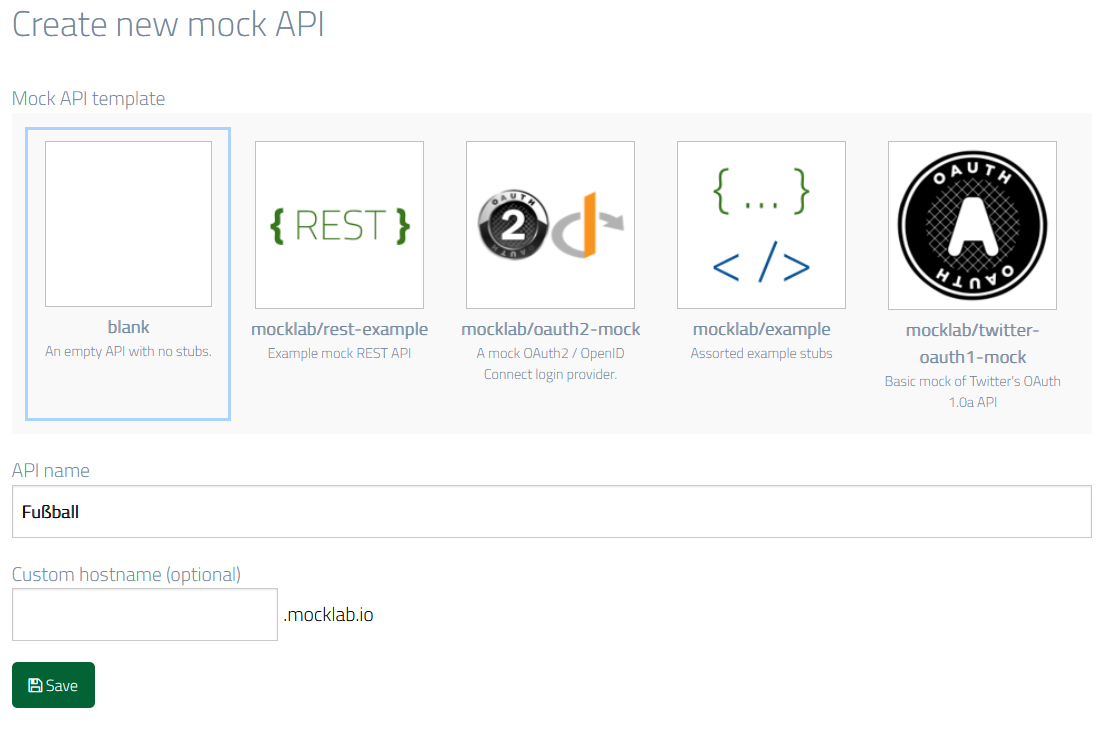
\includegraphics[scale=0.5]{pics/mocklab-tutorial/create-mock-api.PNG}

Die Standard Einstellungen müssten soweit passen, also erstellen wir gleich unseren Stub.
Einfach links auf den 
\includegraphics[scale=0.5]{pics/mocklab-tutorial/new-stub-button.PNG}
klicken und danach in der Menü-Leiste auf 
\includegraphics[scale=0.5]{pics/mocklab-tutorial/new-button.PNG}

Nennen wir den Stub einfach mal Fußballmannschaft und definieren einen sinvollen Pfad für einen GET-Request.
\bigskip

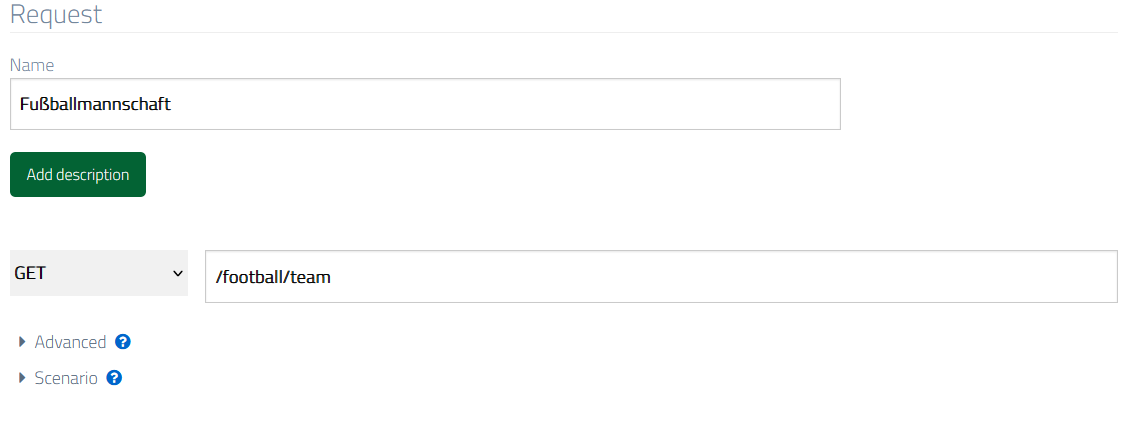
\includegraphics[scale=0.5]{pics/mocklab-tutorial/request.PNG}

\newpage

Dann müssen wir natürlich noch eine Response für unseren Stub erstellen und antworten einfach mal mit einer
JSON-Datei von Paris-Saint-Germain.
\bigskip

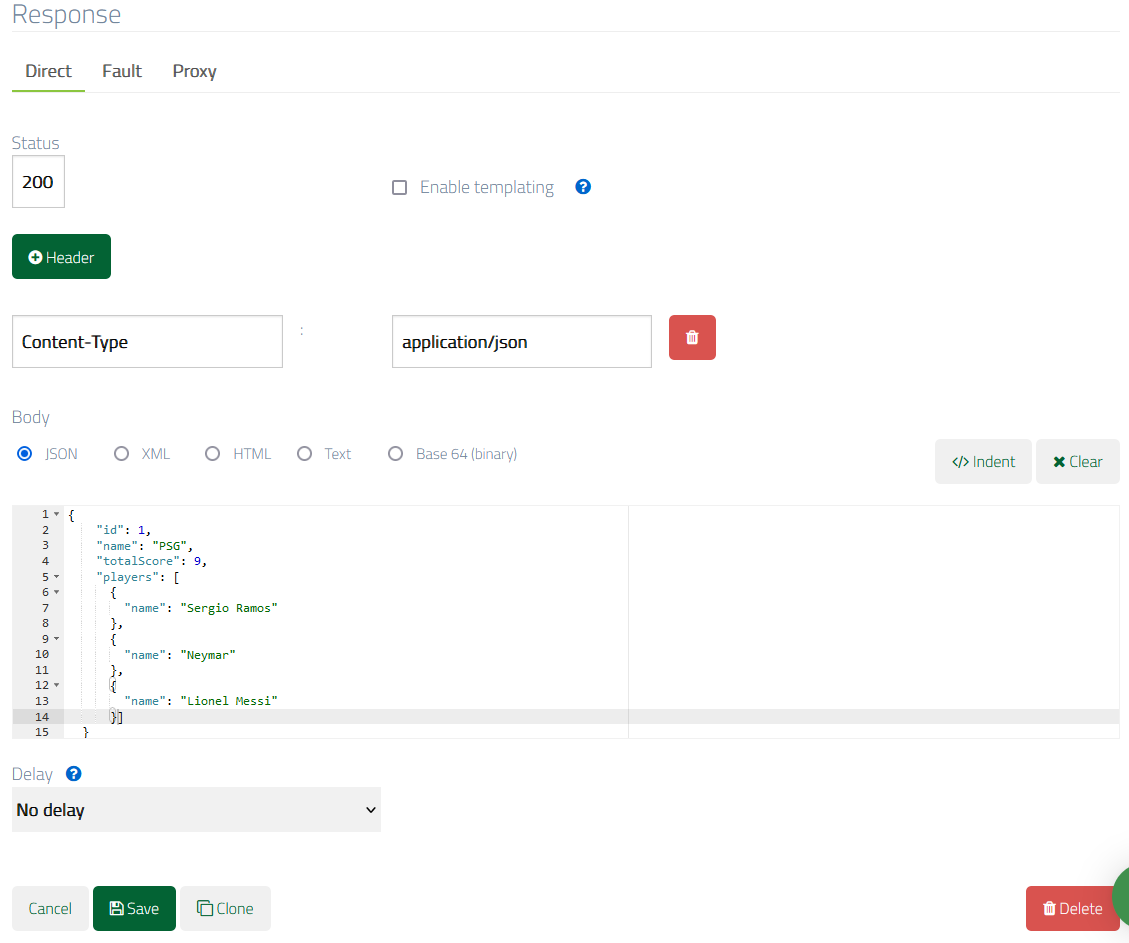
\includegraphics[scale=0.5]{pics/mocklab-tutorial/response.PNG}

Und siehe schon haben wir eine funktionierde Mockup die Daten beispielsweise für eine Frontend-Entwicklung
bereitstellt.
\begin{figure}[h]
    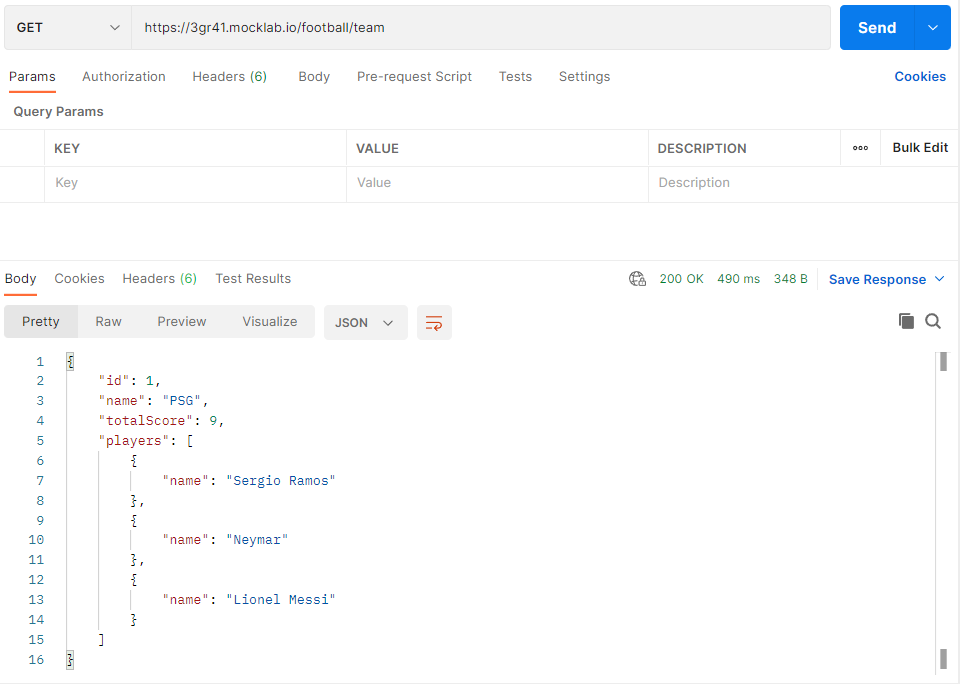
\includegraphics[scale=0.5]{pics/mocklab-tutorial/postman.PNG}
    \caption{Postman Request}
\end{figure}

Da jetzt nun alle Bestandteile und Technologie der App geklärt sind kommt jetzt das Benutzerhandbuch.